\documentclass[9pt]{beamer}

\geometry{paperwidth=160mm,paperheight=120mm}

\usetheme[{titleformat plain}=smallcaps,
           titleformat title=smallcaps,
           titleformat subtitle=regular,
           titleformat section=smallcaps,
           titleformat frame=smallcaps,
           % numbering=fraction,
          ]{metropolis}
% \usepackage{appendixnumberbeamer}

\definecolor{mLightGreen}{HTML}{14B03D}
\definecolor{vpGreen}{HTML}{66c2a5}
\definecolor{vpOrange}{HTML}{fc8d62}
\providecommand{\iRef}[1]{{\color{mLightGreen}\small $[$#1$]$}}

\usepackage{booktabs}
\usepackage[scale=2]{ccicons}

\usepackage{../_style/common}
\usepackage{../_style/defs}

\usepackage{tikz}
\usetikzlibrary{shapes,arrows}
\usepackage{amsmath, bm}
\usepackage{siunitx}
\usepackage{physics,hepnames}
\usepackage{mathtools}
\usepackage{enumitem}
\setenumerate[1]{%
      label=\protect\usebeamerfont{enumerate item}%
      \protect\usebeamercolor[fg]{enumerate item}%
      \insertenumlabel.}
\setitemize{label=\usebeamerfont*{itemize item}%
    \usebeamercolor[fg]{itemize item}
      \usebeamertemplate{itemize item}}

\usepackage{subfig}
\usepackage{colortbl}
\usepackage{multirow}
\usepackage{pifont}

\usepackage{pgfplots}
\usepgfplotslibrary{dateplot}

\usepackage{soul}

\graphicspath{{pictures/}{pictures/backup/}{../2022-ICHEP/pictures/}{../2022-ICHEP/pictures/backup/}}

\title{Theory Predictions}
\subtitle{for PDF fitting}
\date{July, 2022}
\author{\textit{\textbf{Alessandro Candido}}, Felix Hekhorn, Giacomo Magni}
%\institute{N3PDF}
\titlegraphic{
    \raisebox{10pt}[0pt][0pt]{
\includegraphics[width=2.5cm]{../_logos/nnpdf_logo.pdf}}\hspace*{10pt}
    \hfill
    \raisebox{5pt}[0pt][0pt]{
\includegraphics[height=0.8cm]{../_logos/n3pdf_logo.pdf}}\hspace*{10pt}
    
\includegraphics[height=1.3cm]{../_logos/erc_logo1.png}

    \vfill\vspace*{230pt}
    
\includegraphics[height=1cm]{../_logos/unimi_logo.png}\hfill
    
\includegraphics[height=1cm]{../_logos/infn_logo.png}\\
    \vspace*{5pt}
    {
        \fontsize{3pt}{3.5pt}\selectfont
        \begin{center}
            This project has received funding from the European Union's Horizon
            2020 research and innovation programme under grant agreement No
            740006\quad 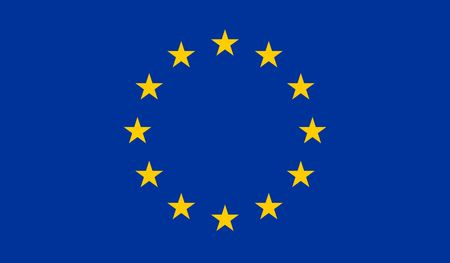
\includegraphics[height=5pt]{../_logos/eu-flag.jpg}
        \end{center}
    }
}

\begin{document}

\maketitle

\setlist[description]{font=\quad\normalfont\bfseries\scshape\space}

\section{\nnpdf{4.0} \iRef{arXiv: 2109.02653}}

\begin{frame}{\nnpdf{4.0}}
    \begin{center}
            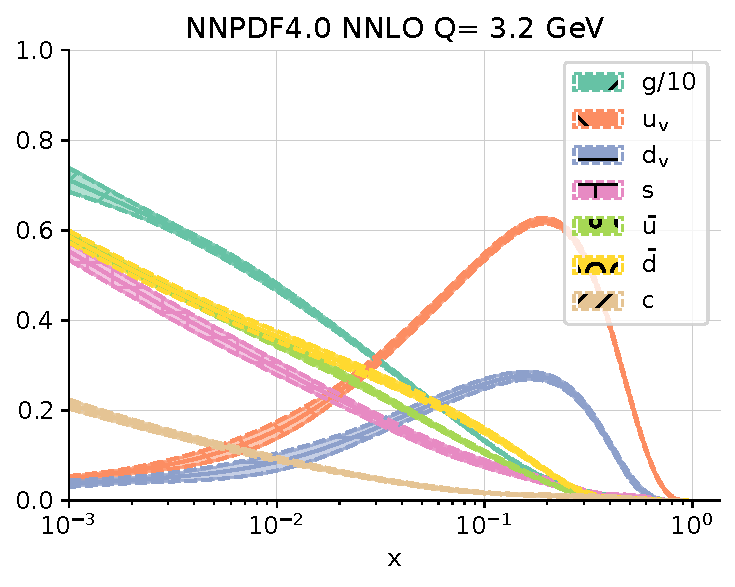
\includegraphics[width=.49\linewidth]{pdfs_pdg_Qs0_plot_flavours}
            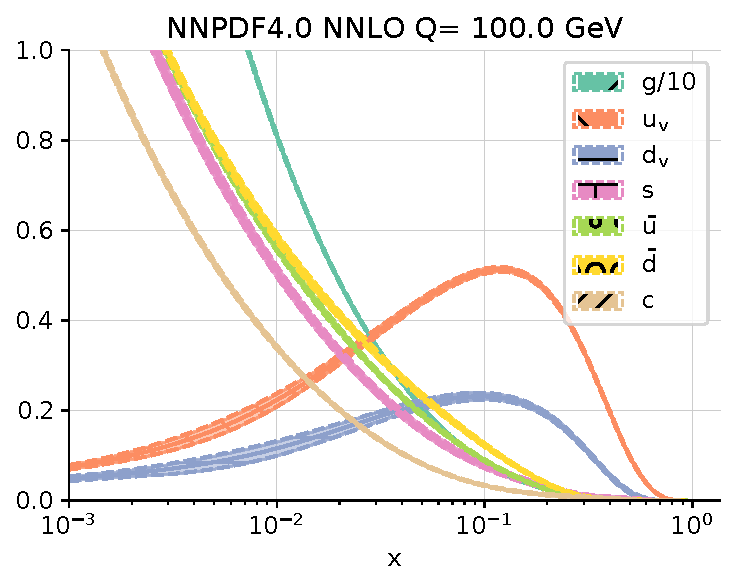
\includegraphics[width=.49\linewidth]{pdfs_pdg_Qs1_plot_flavours}
    \end{center}
\end{frame}

\begin{frame}{\nnpdf{4.0}: Highlights}
    \begin{columns}
        \begin{column}{0.4\textwidth}
            \begin{description}
                \item[methodology] new Neural Network, based on widely
                    supported, industry-level library, with further tests and
                    machine-learning inspired improvements
                \item[data] more data from \lhc, and a massive increment in the
                    number of processes (jets, dijets, single top, top pair,
                    \dots)
                \item[errors] a consequential great reduction in uncertainty
                \item[backward compatible] preserving compatibility with
                    \nnpdf{3.1}
                \item[public code] code public \iRef{arXiv: 2109.02671} and
                    documented
                \begin{itemize}
                    \item \enquote{make your own \nnpdf{}!}
                \end{itemize}
            \end{description}
        \end{column}
        \begin{column}{0.5\textwidth}
            \begin{center}
                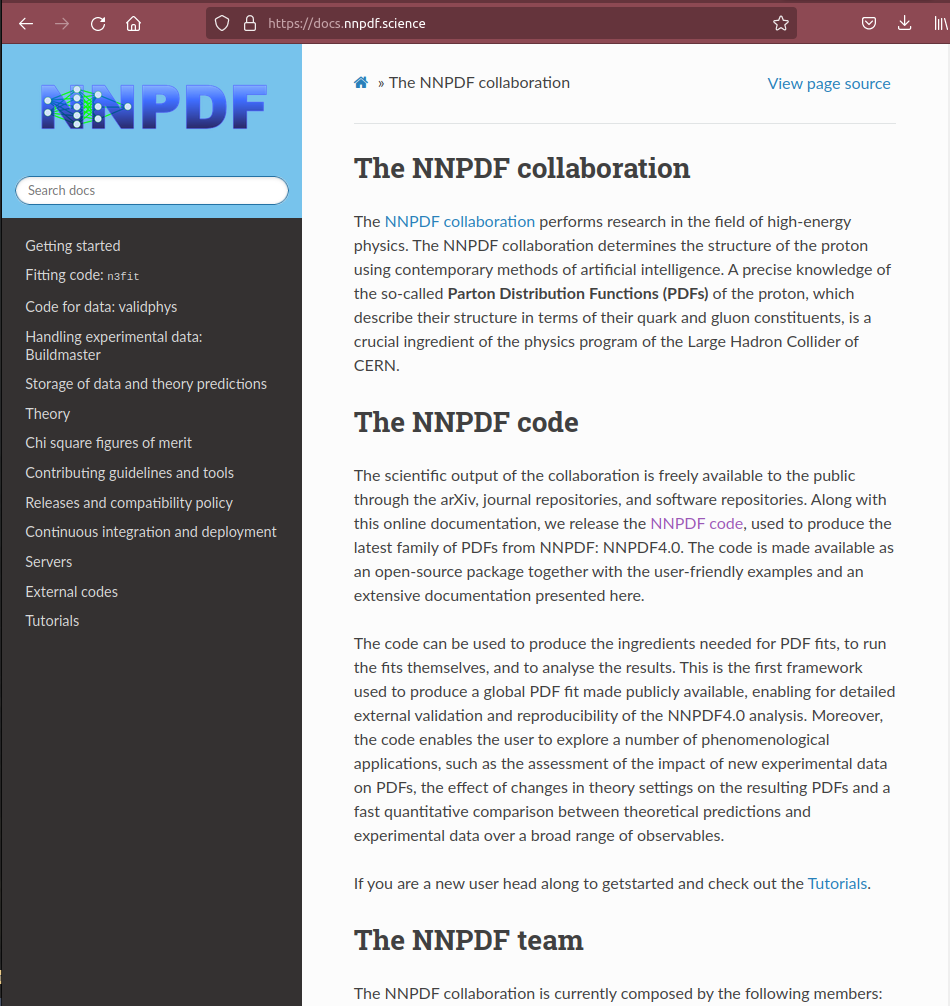
\includegraphics[width=1.1\textwidth]{nnpdf-docs}
            \end{center}
        \end{column}
    \end{columns}
\end{frame}

\begin{frame}{\nnpdf{4.0}: Theory?}
    Mostly the same (not really: K-factors recomputed, a lot of new processes).
    \vspace*{10pt}
    \begin{center}
        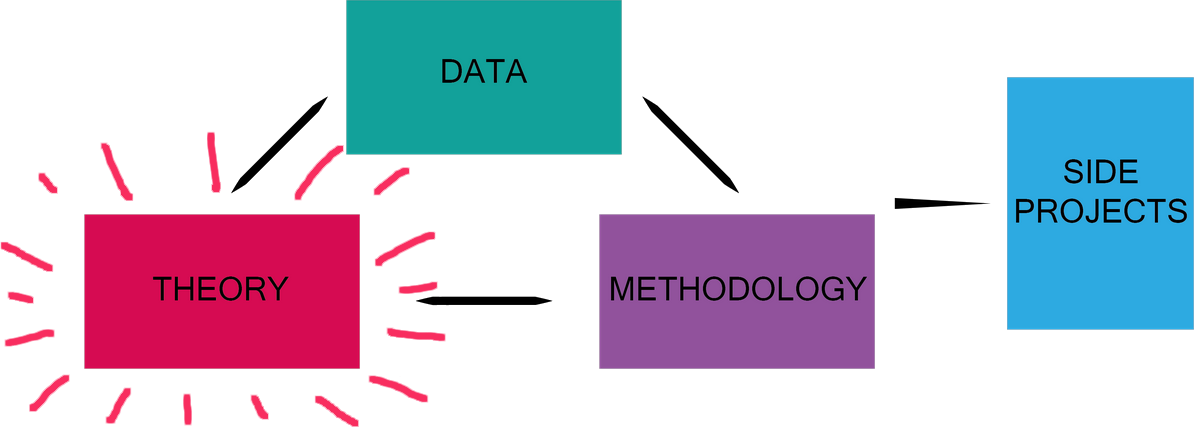
\includegraphics[width=0.7\linewidth]{organization}
    \end{center}
    \vspace*{10pt}
    But main providers\footnote{
        In particular it is one: \apfel, and the associated \apfelcomb.
    } (DIS, evolution, FTDY) are the exact same of \nnpdf{3.1}.
\end{frame}

\section{\eko{} \iRef{arXiv: 2202.02338}}

\begin{frame}{\eko{} Definition}
    \begin{center}
            
\includegraphics[width=.35\linewidth]{eko}
    \end{center}

    The main purpose is to solve \textbf{\dglap}\ equations:
    \begin{equation*}
            \muF^2 \dv{\vb f}{\muF^2}{}(\muF^2) = \vb P (a_s(\muR^2),\muF^2) \otimes \vb f(\muF^2)
    \end{equation*}

    These equations define a set of linear operators $\vb E(\muF^2 \leftarrow
    \mu_{F,0}^2)$ on \textbf{\pdf}\ sets
    \begin{equation*}
            \vb f(\muF^2) = \vb E(\muF^2 \leftarrow \mu_{F,0}^2) \otimes \vb f(\mu_{F,0}^2)
    \end{equation*}

    \vspace*{15pt}
    \begin{center}
            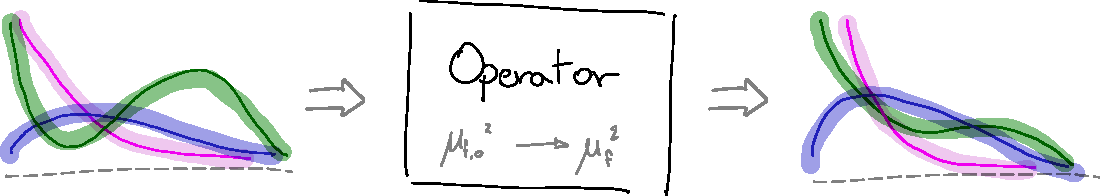
\includegraphics[width=0.7\linewidth]{ev-op}
    \end{center}
\end{frame}

\begin{frame}{Operator Advantage}
    \vspace*{15pt}
    Independent of boundary condition $\to$ \pdf{} fitting

    \vspace*{25pt}
    \begin{center}
            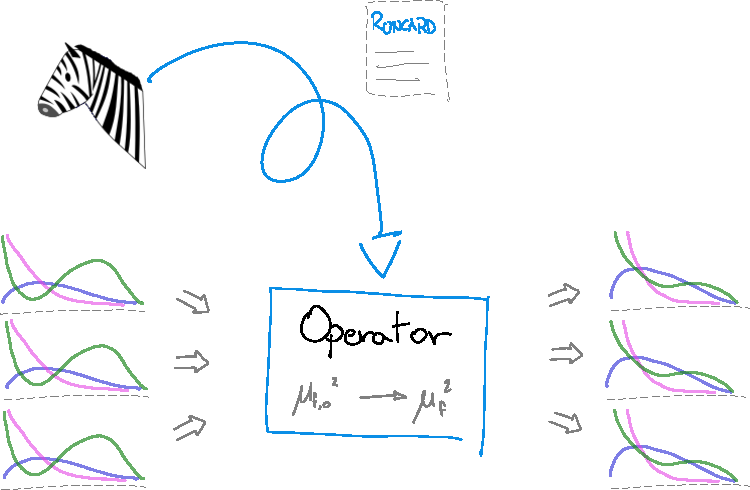
\includegraphics[width=0.7\linewidth]{compute-ev-op-zebra}
    \end{center}
\end{frame}

\begin{frame}{User-friendly Mellin Space}
    \vspace*{15pt}
    \textbf{Solved in Mellin} ($N$-) space, but the operator is recasted in
    \textbf{$x$-space}.

    \vspace*{15pt}
     Via piecewise Lagrange-interpolation:
     \begin{description}
         \item[input] \pdf\ is interpolated with polynomials, and
             \textit{\textbf{analytically}} Mellin transformed
         \item[output] \pdf\ is given on grid points, and Mellin inverted
             \textit{\textbf{numerically}}
     \end{description}

    \vspace*{25pt}
    \begin{center}
            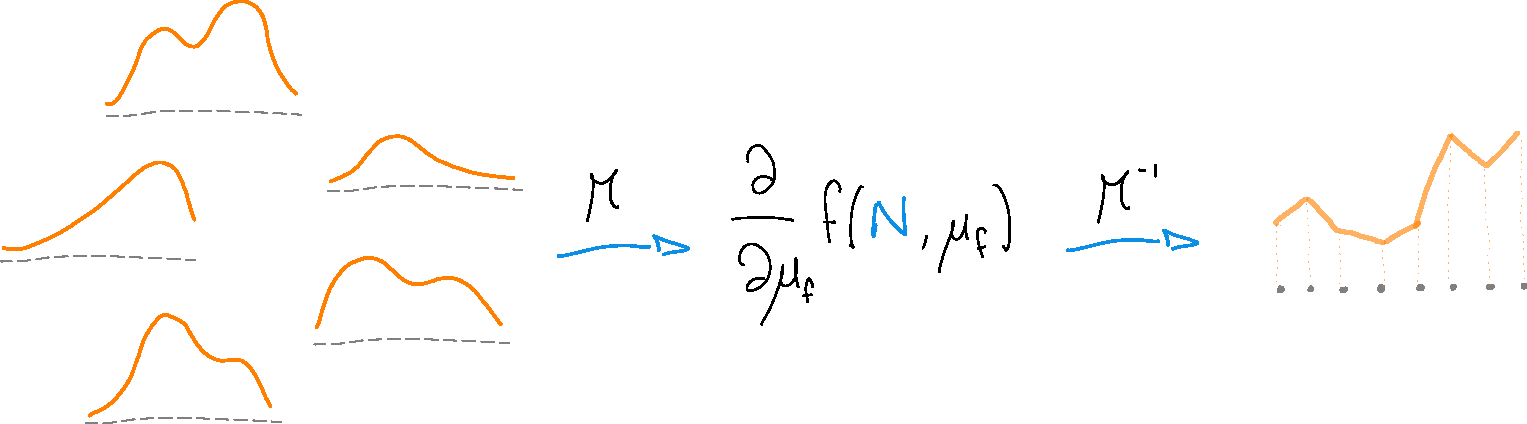
\includegraphics[width=0.9\linewidth]{mellin}
    \end{center}
\end{frame}

\begin{frame}{Original Physics}

    \begin{columns}
        \begin{column}{0.4\textwidth}
            Consistent evolution of \textbf{intrinsic} heavy quark
            distributions.
        \end{column}
        \begin{column}{0.5\textwidth}
            \begin{center}
                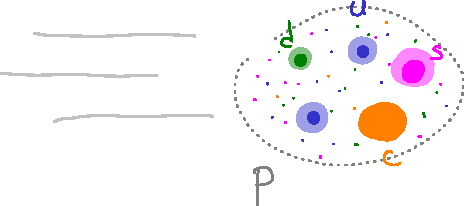
\includegraphics[width=0.9\linewidth]{intrinsic}
            \end{center}
        \end{column}
    \end{columns}

    \vspace*{10pt}
    \begin{columns}
        \begin{column}{0.5\textwidth}
            \begin{center}
                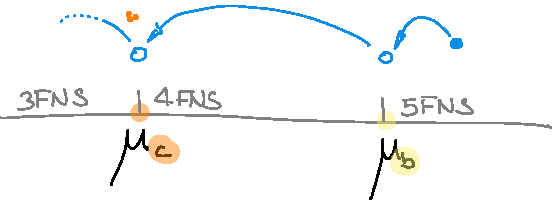
\includegraphics[width=0.9\linewidth]{back-vfns}
            \end{center}
        \end{column}
        \begin{column}{0.4\textwidth}
            Full \textbf{backward \vfns{}} evolution (i.e.\ across thresholds
            and with intrinsic).
        \end{column}
    \end{columns}

    \vspace*{35pt}
    And more to come (\mhou, \qed, \nnnlo, \dots).
\end{frame}

\section{Intrinsic Charm in the Proton \iRef{in press}}

\begin{frame}{Intrinsic Charm: Strategy}
    Based on \nnpdf{4.0} \iRef{\href{https://arxiv.org/abs/2109.02653}{arxiv:2109.02653}}.

    \begin{center}
        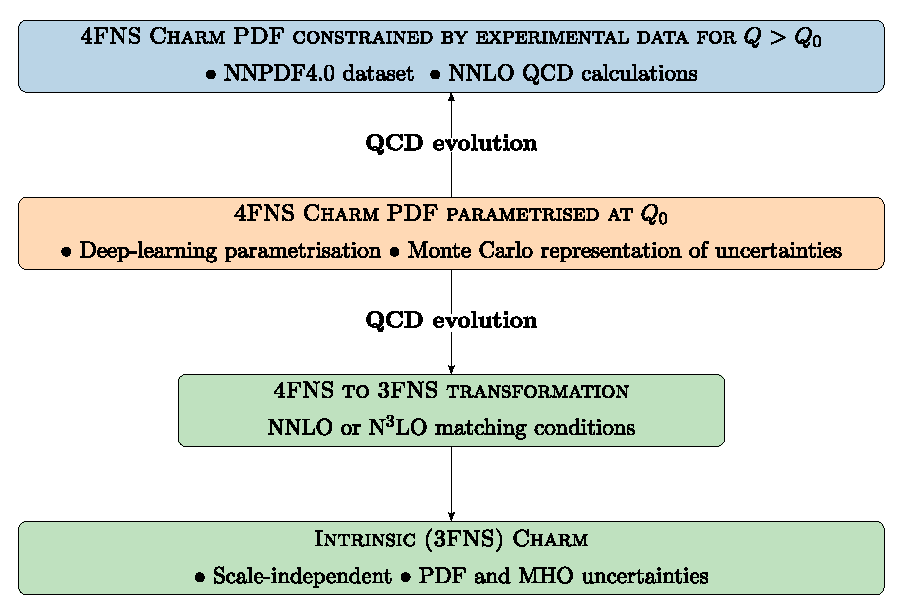
\includegraphics[scale=.6]{strategy}
    \end{center}

    \textsc{\textbf{Intrinsic}}\quad it is the charm PDF in the \textbf{3FNS},
    where the charm is actually considered \alert{\textbf{massive}}
    {\footnotesize (and consequently \textit{factorization scale independent}
    -- collinear divergencies are protected by the mass)}
\end{frame}

\begin{frame}{Matching Conditions and Backward Evolution}
    \vspace*{10pt}

    For (forward) evolution across a matching scale $\mu_h^2$:
    \begin{equation*} 
    \mathbf{f}^{(n_f+1)}(\mu_{F,1}^2) =
    \left[\mathbf{E}^{(n_f+1)}(\mu_{F,1}^2\leftarrow \mu_{h}^2)
            {\mathbf{R}^{(n_f)}}
            \mathbf{A}^{(n_f)}(\mu_{h}^2)
    \mathbf{E}^{(n_f)}(\mu_{h}^2\leftarrow \mu_{F,0}^2) \right]
            \times \mathbf{f}^{(n_f)}(\mu_{F,0}^2)
    \end{equation*}
    \vspace*{5pt}

    The \textbf{Operator Matrix Element} (\ome) $\mathbf{A}^{(n_f)}(\mu_{h}^2)$
    is partially known up to \alert{\textbf{\nnnlo}}.

    \begin{center}
        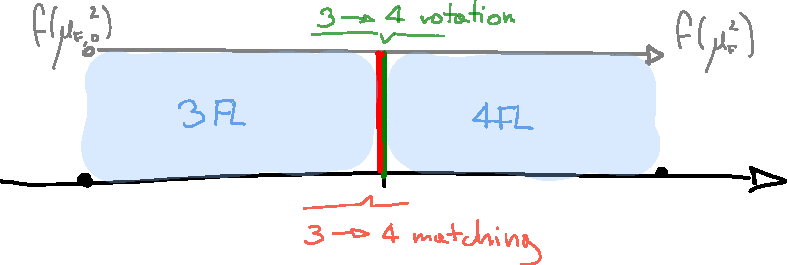
\includegraphics[scale=.7]{vfns-details}
    \end{center}
    \vspace*{5pt}

    \alert{\textbf{Inverse operator}} (the \ome can be inverted either
    \textit{perturbatively} or \textit{numerically})
    \begin{center}
        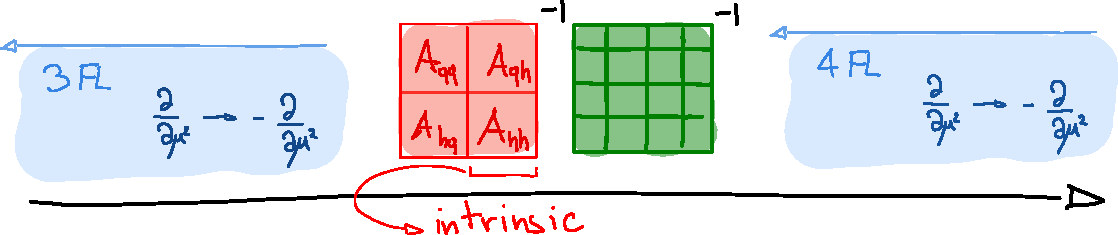
\includegraphics[scale=.7]{vfns-back-details}
    \end{center}
\end{frame}

\begin{frame}{Intrinsic Charm: \pdf{} plot}
    \begin{center}
        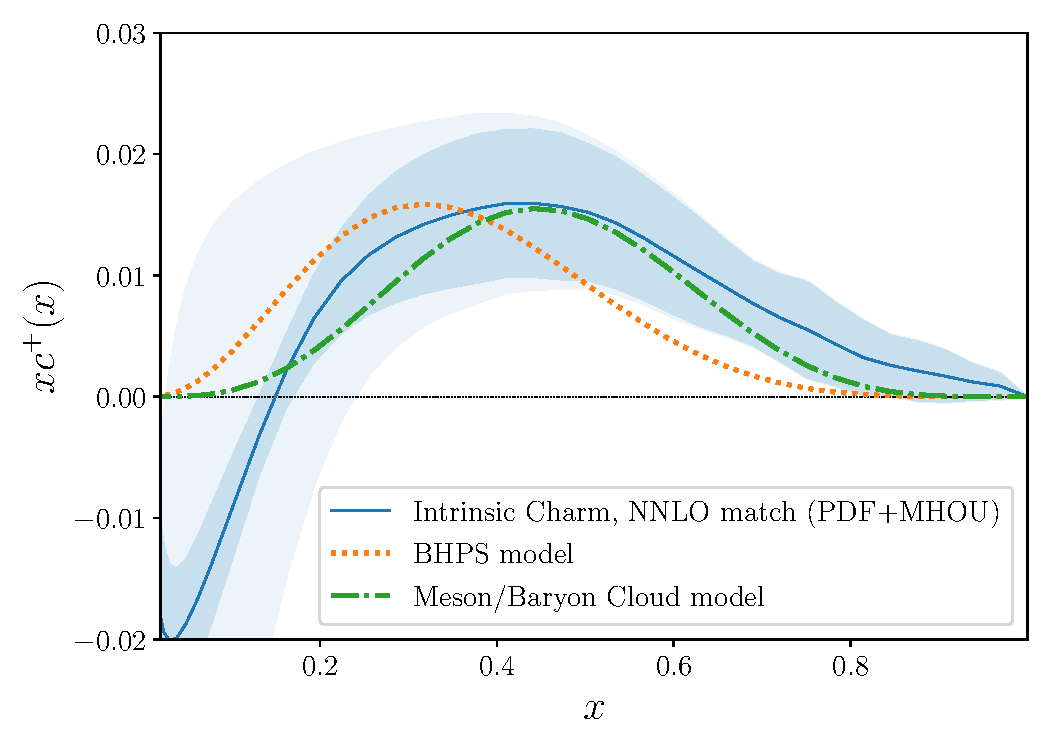
\includegraphics[width=.7\linewidth]{nf3_to_models.pdf}\\
        \vspace*{-5pt}
        \quad\iRef{\href{https://doi.org/10.1016/0370-2693(80)90364-0}{BHPS}}
        or \iRef{\href{https://doi.org/10.1103/PhysRevD.89.074008}{Meson/Baryon
        Cloud Model}}
    \end{center}
    \vspace*{10pt}

    \textsc{\textbf{Message}} In \textbf{\alert{3FNS}} a \textbf{valence-like
    peak} is present.

	\begin{itemize}
        \item for \textbf{$x\leq 0.2$} the perturbative
            \textit{\textbf{uncertainties}} are quite \textit{\textbf{large}}
        \item the carried \textit{\textbf{momentum fraction}} is within \textbf{1\%}
	\end{itemize}
\end{frame}

\begin{frame}{Intrinsic Charm: LHCb and Significance}
	\begin{center}
		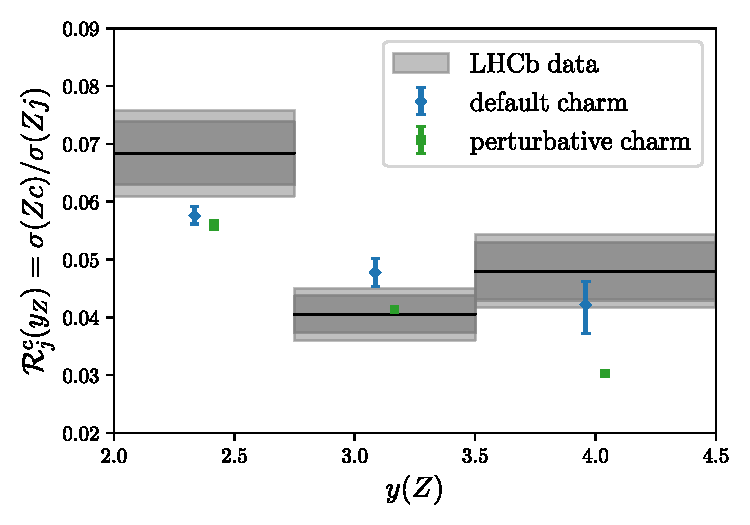
\includegraphics[width=.47\linewidth]{lhcb-zcharm-pheno}%
		\quad%
		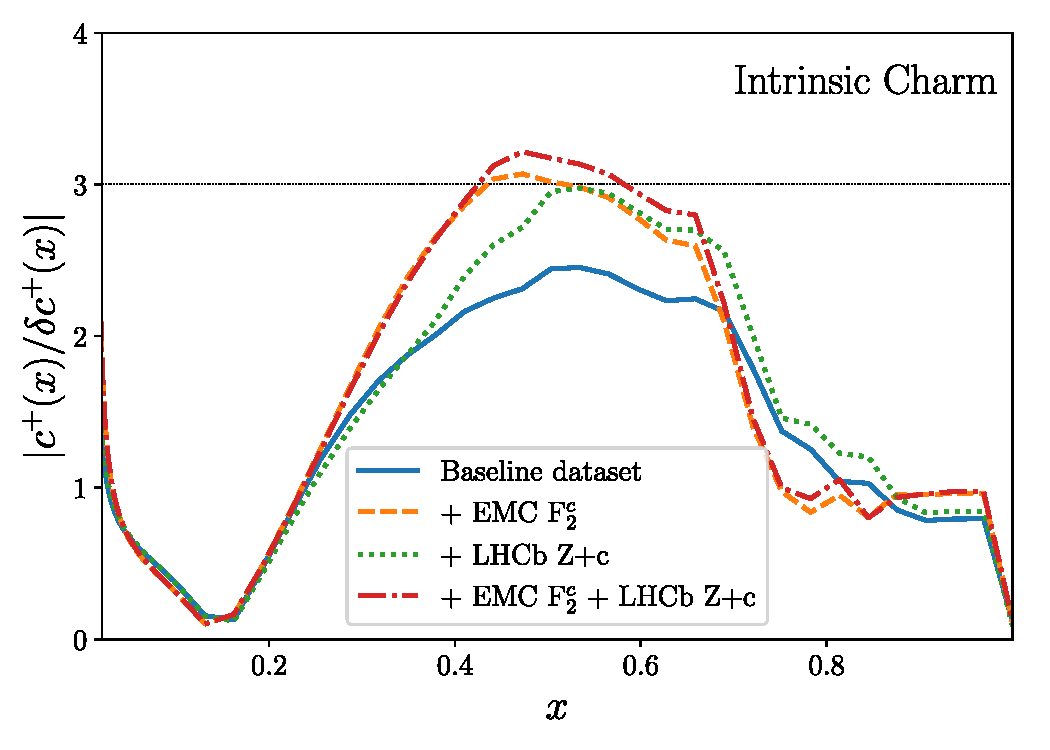
\includegraphics[width=.47\linewidth]{pull_baseline_EMC_LHCb_Zc}
	\end{center}

    We found a $\bm{3\sigma}$ evidence of \alert{\textbf{intrinsic charm}}
	\begin{itemize}
		\item match better recent \textbf{LHCb} Z+c measurement \iRef{\href{https://doi.org/10.1103/PhysRevLett.128.082001}{PRL128-082001}}
		\item result is \textbf{stable} with mass variation, dataset variation
	\end{itemize}
\end{frame}


\section{\yadism{} \iRef{in preparation}}

\begin{frame}{\yadism{} Physics Features}
    \vspace*{5pt}
	\begin{center}
		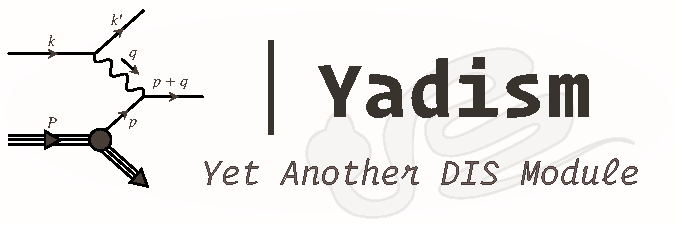
\includegraphics[width=.4\linewidth]{yadism.pdf}
	\end{center}

    \vspace*{5pt}
    \begin{columns}
        \begin{column}{0.5\textwidth}
            \begin{center}
                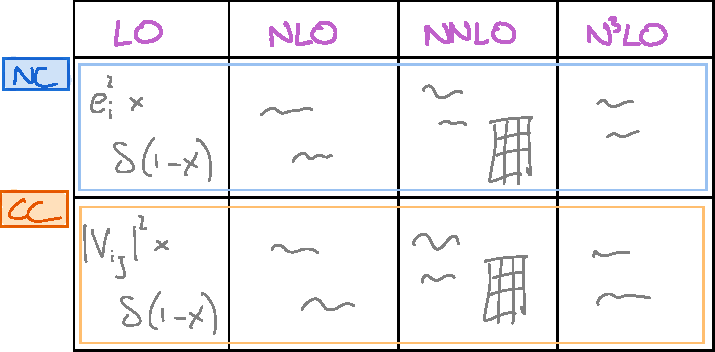
\includegraphics[width=0.6\linewidth]{dis-db}
            \end{center}
        \end{column}
        \begin{column}{0.4\textwidth}
            DIS \textbf{\alert{coefficient function} database}
        \end{column}
    \end{columns}

    \vspace*{5pt}
    \begin{columns}
        \begin{column}{0.4\textwidth}
            \textbf{Independent} of \textbf{boundary} condition $\to$ \pdf fitting.
        \end{column}
        \begin{column}{0.5\textwidth}
            \begin{center}
                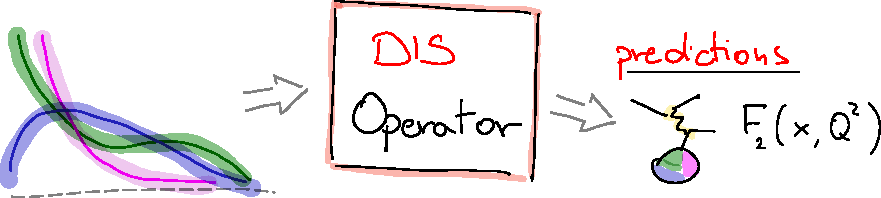
\includegraphics[width=\linewidth]{dis-op}
            \end{center}
        \end{column}
    \end{columns}

    \vspace*{15pt}
    \begin{center}
        Several other features: \textbf{TMC}, multiple \textbf{FNS}, generic
        matching scales, interpolation, \dots
    \end{center}

    \vspace*{15pt}
    Constant benchmark against \apfel. 
\includegraphics[width=1em]{green-tick}\\
    Multiple benchmarks against \qcdnum. 
\includegraphics[width=1em]{green-tick}\\
    Benchmark with original \fonll. 
\includegraphics[width=1em]{green-tick}
\end{frame}

\begin{frame}{DIS coefficients}
    \vspace*{25pt}

    \begin{columns}
        \begin{column}{0.5\textwidth}
            \begin{table}[h!]
                \large
                \centering
                \begin{tabular}{c | c c c } 
                    \nlo & light & heavy & intrinsic\\
                    \hline
                    NC & \cellcolor{green!25}\checkmark 
                       & \cellcolor{green!25}\checkmark 
                       & \cellcolor{green!25}\checkmark\\
                    CC & \cellcolor{green!25}\checkmark
                       & \cellcolor{green!25}\checkmark
                       & \cellcolor{blue!25}\checkmark\\
                    \nnlo & & &\\
                    \hline
                    NC & \cellcolor{green!25}\checkmark
                       & \cellcolor{blue!25}partially tabulated
                       & \cellcolor{red!25}\ding{55}\\
                    CC & \cellcolor{green!25}\checkmark
                       & \cellcolor{yellow!25}tabulated
                       & \cellcolor{red!25}\ding{55}\\
                    \nnnlo & & &\\
                    \hline
                    NC & \cellcolor{yellow!25}\checkmark
                       &  & \\
                    CC & \cellcolor{yellow!25}\checkmark
                       &  & \\
                \end{tabular}
            \end{table}
            + \fonll\ (cf. \textit{matching conditions})
        \end{column}
        \begin{column}{0.4\textwidth}
            There is even another couple of levels of nesting:
            
            \begin{description}
                \item[Projections] $F_2$, $F_L$, and $F_3$
                \item[Channels] non-singlet, singlet, gluon
            \end{description}

            \vspace*{10pt}
            {
                \footnotesize
                But up to \nnlo\ everything is equally available (while at
                \nnnlo\ it is not always true).
            }
        \end{column}
    \end{columns}

    \vspace*{10pt}

    So NC is currently implemented up to NNLO
    \iRef{\href{https://doi.org/10.1016/j.nuclphysb.2005.06.020}{VVM05}
    \href{https://doi.org/10.1016/j.physletb.2004.11.063}{MVV05}
    \href{https://doi.org/10.1016/S0550-3213(00)00045-6}{MV00}}
    light and NLO heavy \iRef{\href{https://arxiv.org/abs/1910.01536}{Hek19}}
    (i.e. both $O(a_s^2)$).
    Same for CC light
    \iRef{\href{https://doi.org/10.1016/j.nuclphysb.2007.09.022}{MRV08}
    \href{https://doi.org/10.1016/j.nuclphysb.2009.01.001}{MVV09}} and heavy
    (for which implementation is currently in progress).

    For both processes \textit{intrinsic} contributions are accounted at NLO.
    
    \vspace*{15pt}
    {
        \footnotesize
        \begin{flushright}
            \begin{tabular}{c c c c c} 
                \cellcolor{green!25}available
                    & \cellcolor{blue!25}updated
                    &\cellcolor{yellow!25}not yet implemented
                    &\cellcolor{red!25}missing
                    & not planned\\
                \hline
            \end{tabular}
        \end{flushright}
    }
\end{frame}

\begin{frame}{Comparison \yadism{} against \apfel{}}
    \begin{center}
        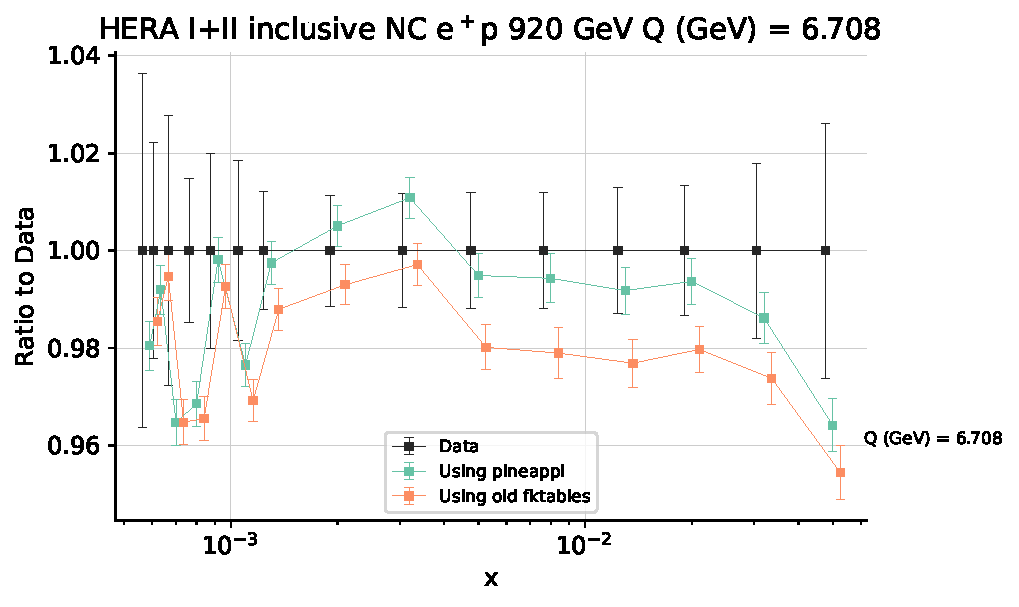
\includegraphics[width=.47\linewidth]{
            matched_datasets_from_dataspecs14_dataset_report_Datanorm_plot_fancy_dataspecs_11.pdf
        }
        \quad
        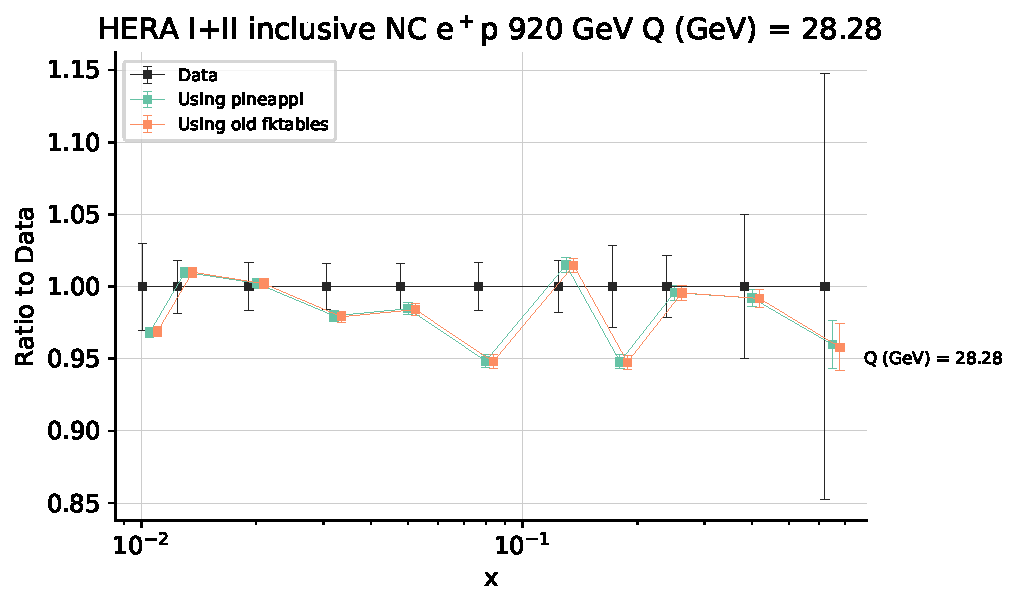
\includegraphics[width=.47\linewidth]{
            matched_datasets_from_dataspecs14_dataset_report_Datanorm_plot_fancy_dataspecs_23.pdf
        }
        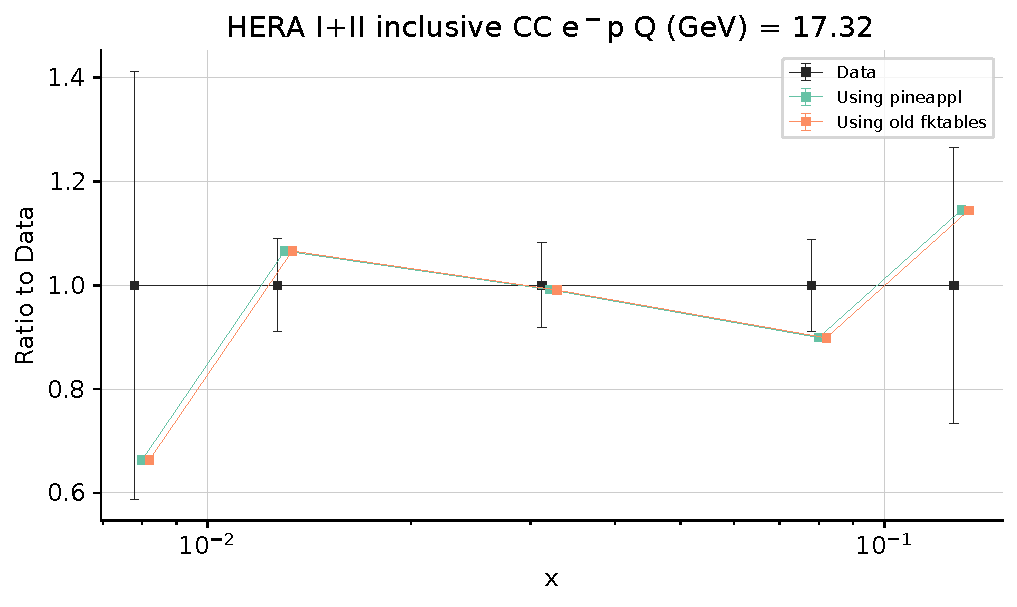
\includegraphics[width=.47\linewidth]{
            matched_datasets_from_dataspecs4_dataset_report_Datanorm_plot_fancy_dataspecs_0.pdf
        }
        \quad
        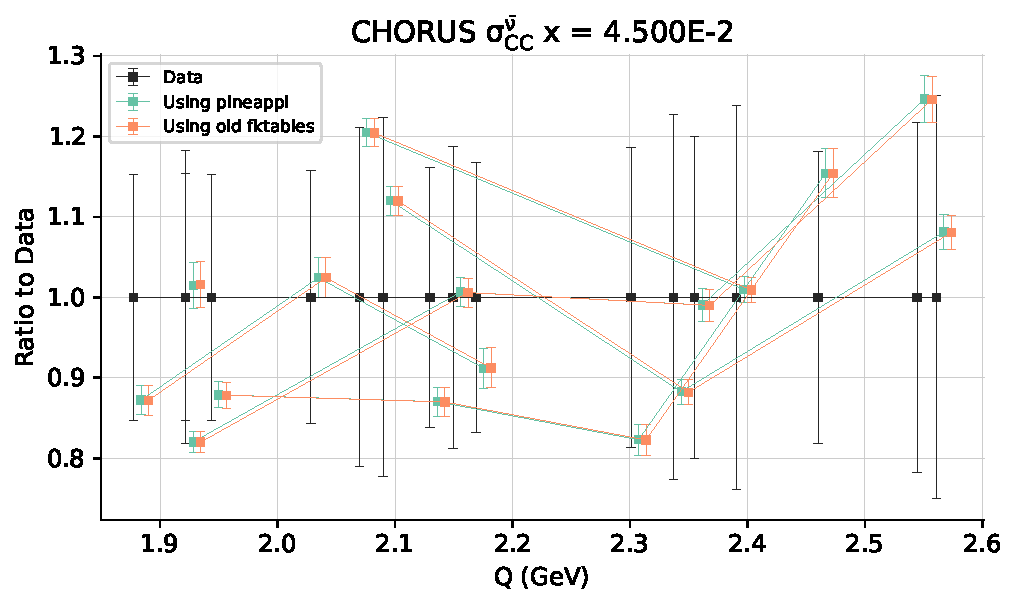
\includegraphics[width=.47\linewidth]{
            matched_datasets_from_dataspecs2_dataset_report_Datanorm_plot_fancy_dataspecs_0.pdf
        }


        % {\color{vpGreen} green}, \enquote{pineappl} = \yadism{} vs. {\color{vpOrange} orange}, \enquote{old} = \apfel{}
    \end{center}
\end{frame}

\section{Theory Prediction Pipeline}

\begin{frame}{New Theory Prediction Pipeline}
	\begin{center}
		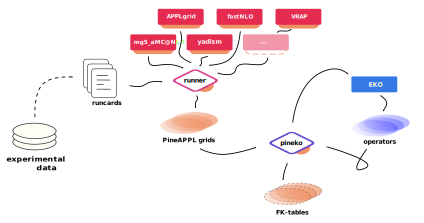
\includegraphics[width=.8\linewidth]{fk}
	\end{center}

	\begin{itemize}
        \item We're about to develop a new pipeline for theory predictions
            around \pineappl{}
            \iRef{\href{https://arxiv.org/abs/2008.12789}{arXiv:2008.12789}}
		\item both, \eko and \yadism, are interfaced with \pineappl
        \item \pineappl also has interfaces to \madgraph, \appl, \fastnlo
	\end{itemize}

    \vspace*{10pt}
    \textbf{\textsc{Goal}}\quad produce \fk tables used in \pdf fitting
\end{frame}

\section{Summary}

\begin{frame}{Summary: theory}
    I hope you enjoyed the effort of converting words in pictures. But now is
    the time of a few words\dots
    \vspace*{10pt}

    \begin{itemize}
        \item \textbf{computing expressions \alert{\textit{is not the end of
            the story}}}
        \item Monte Carlo generators and other providers (e.g.\ \yadism{}) are \textit{essential}
        \begin{itemize}
            \item but \textbf{not enough} for a \pdf{}-like fit (including $\alpha_s$)
        \end{itemize}
        \item predictions have to be agnostic to the fitted object, to avoid
            recomputation $\to$ we need \alert{\textbf{interpolation grids}}
            {\footnotesize note that \textbf{interpolation} \textbf{here is not
            a compromise}, since unknown functions like \pdf{}s are
            \textbf{defined through} interpolation}
        \item \pineappl is such a format, providing extensive tooling and bindings
        \item \textbf{\alert{interfacing}} is \textbf{crucial}:
            developing all this software is \textit{expensive}, so the
            community can not pay the price of doing it over and over $\to$
            tools have to become \textbf{modular} and \textbf{interoperable}
        \item \textbf{\alert{file}-base exchange}, with clear specification of
            data format helps a lot
        \begin{itemize}
            \item preferably based on \textit{wide-spread and supported \textbf{data
                serialization formats}}, e.g.\ \texttt{JSON} or \texttt{hdf5}, in
                order to make them usable by as many programs (and programming
                languages) as possible in the cheapest way
            \item \lhapdf is a good example
        \end{itemize}
    \end{itemize}
\end{frame}

\begin{frame}{Summary: our tools}
    Why should one use:
    \begin{description}
        \item[\eko?] because:
            \begin{itemize}
                \item it produces \enquote{out of the box} \textbf{operators}
                \item the operators can be immediately used \textbf{together with grids}
                \item it joins advantages of \textbf{$x$ and $N$ space}
                \item it is getting more and \textbf{more physics
                    features} (intrinsic, backward \vfns, \qed, \nnnlo)
            \end{itemize}
        \item[\yadism?] because:
            \begin{itemize}
                \item direct production \textbf{DIS grids}
                \item extensive (and extended) database of \textbf{coefficient
                    functions}
                \item thorough implementation of \textbf{FNS} (and more\dots)
            \end{itemize}
        \item[Pipeline?] because:
            \begin{itemize}
                \item it makes \textbf{easy, flexible, and reproducible}
                \item to produce \textbf{performant theory} predictions for PDF fitting
            \end{itemize}
                 \end{description}

    \vspace*{15pt}
    \alert{\textbf{Intrinsic charm}} itself is a \textit{joint} product of \eko
    and \textbf{\nnpdf{4.0}} efforts.
\end{frame}

\begin{frame}[standout]
    Thank you for listening!
\end{frame}

\appendix

\section{\eko}

\subsection{Benchmarks}
\begin{frame}{\eko{} \apfel{} benchmark}
	\begin{center}
		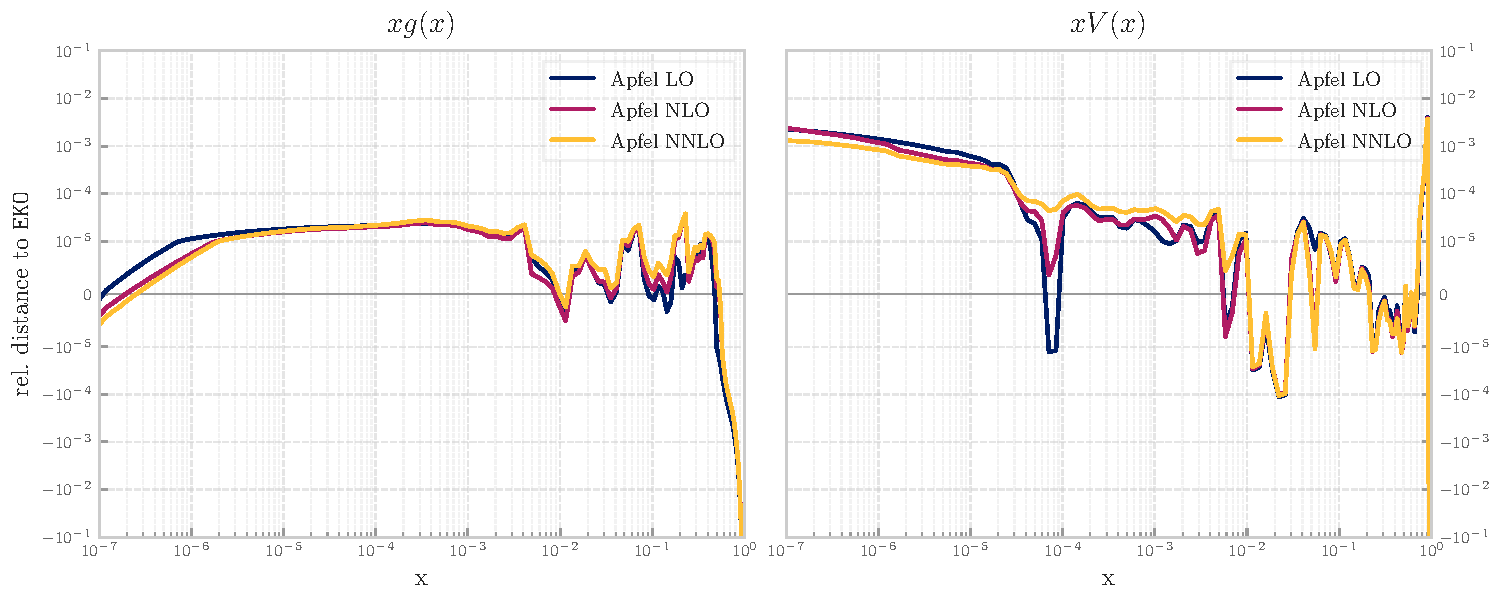
\includegraphics[width=\linewidth]{Apfel_bench_pto.pdf}
	\end{center}
\end{frame}
\begin{frame}{\eko{} \pegasus{} benchmark}
	\begin{center}
		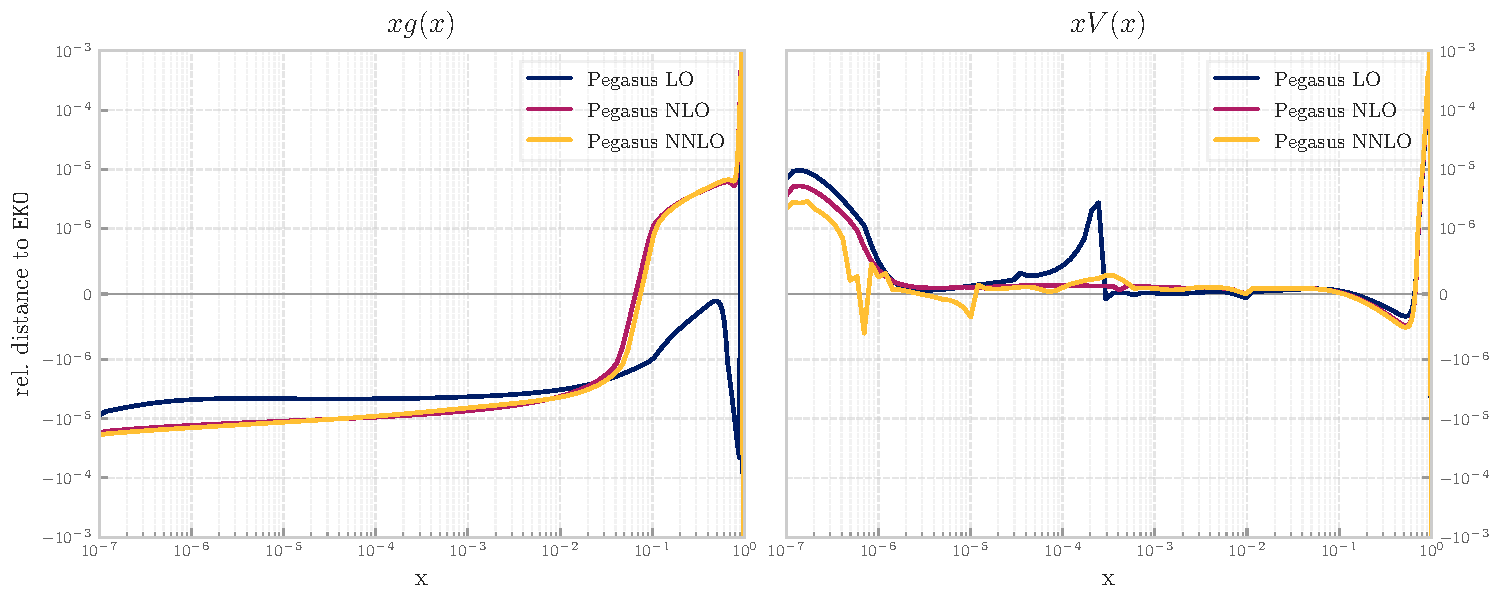
\includegraphics[width=\linewidth]{Pegasus_bench_pto.pdf}
	\end{center}
\end{frame}
\begin{frame}{\eko{} \lha{} benchmark: $g$ and $\Sigma$}
	\begin{center}
		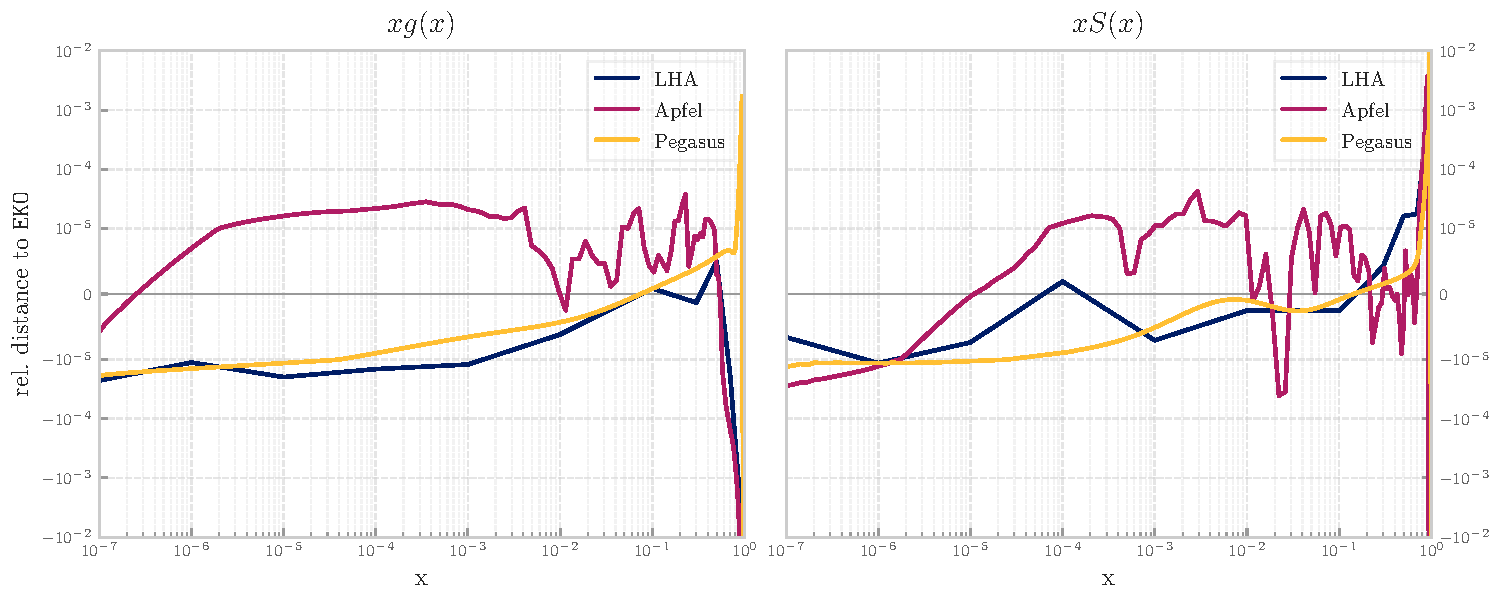
\includegraphics[width=\linewidth]{lha_bench_g_S.pdf}
	\end{center}
\end{frame}
\begin{frame}{\eko{} \lha{} benchmark: $V$ and $V_3$}
	\begin{center}
		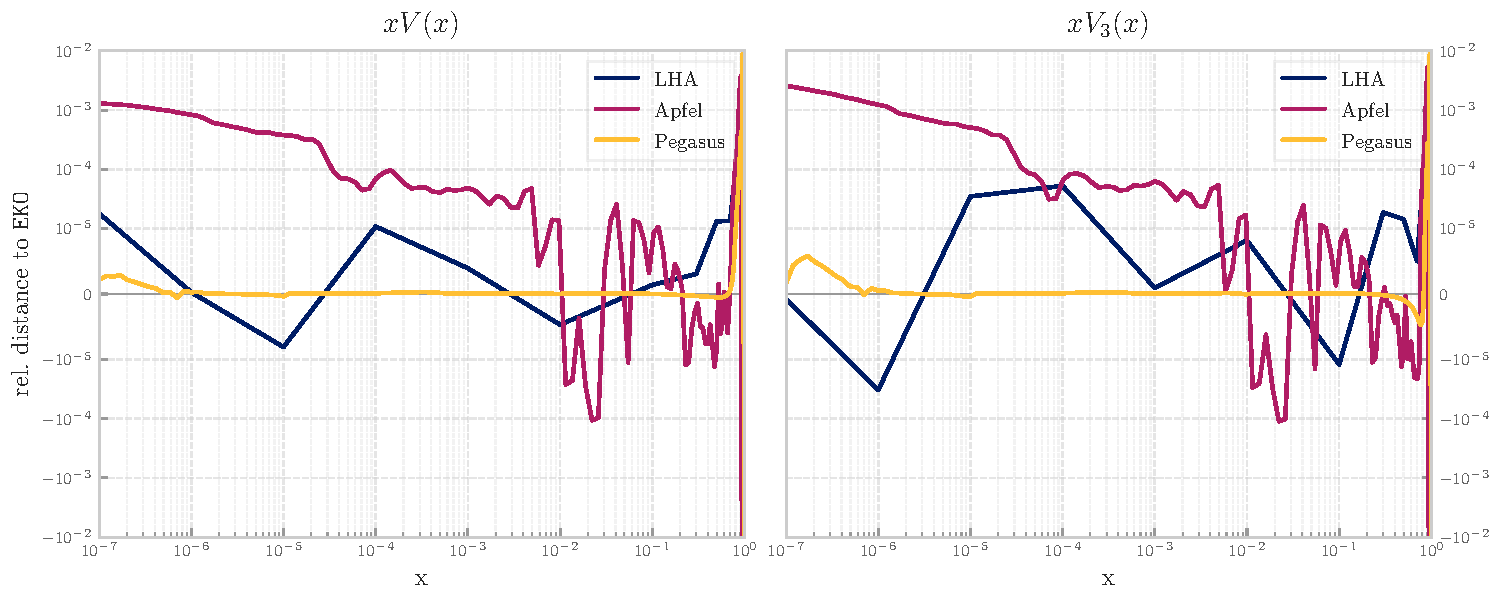
\includegraphics[width=\linewidth]{lha_bench_V_V3.pdf}
	\end{center}
\end{frame}
\begin{frame}{\eko{} \lha{} benchmark: $T_3$ and $T_8$}
	\begin{center}
		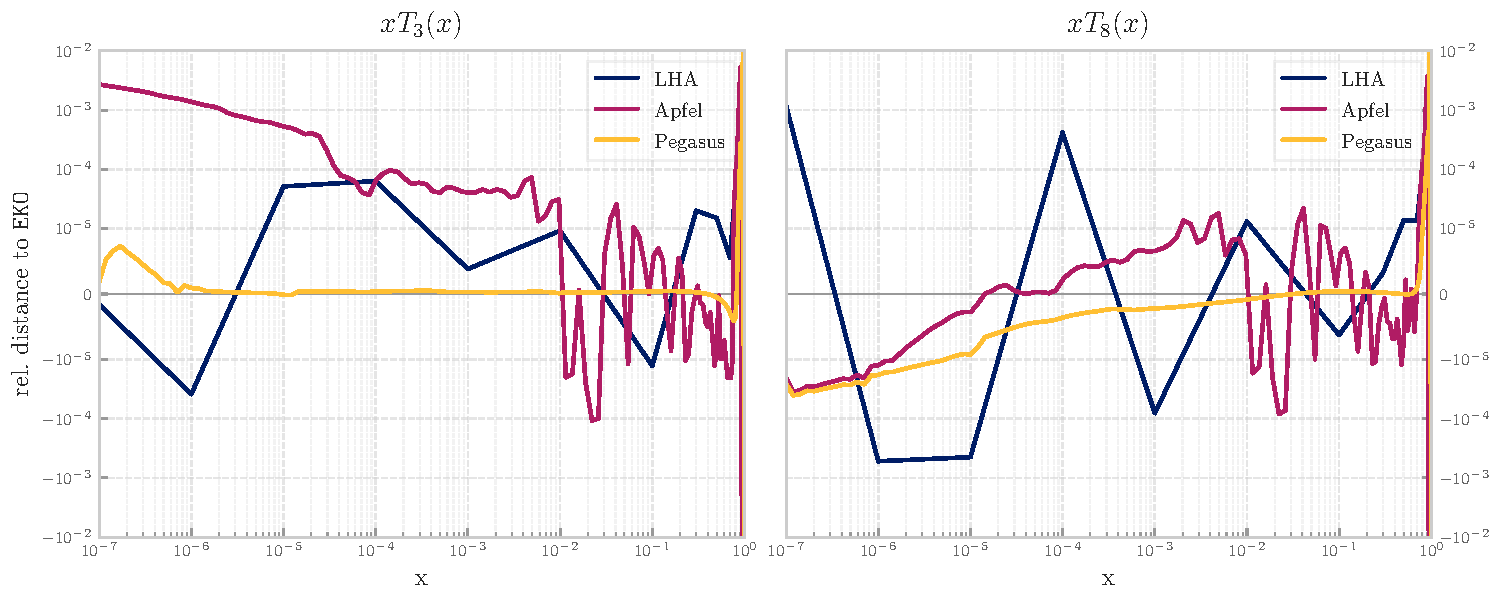
\includegraphics[width=\linewidth]{lha_bench_T3_T8.pdf}
	\end{center}
\end{frame}
\begin{frame}{\eko{} \lha{} benchmark: $T_{15}$ and $T_{24}$}
	\begin{center}
		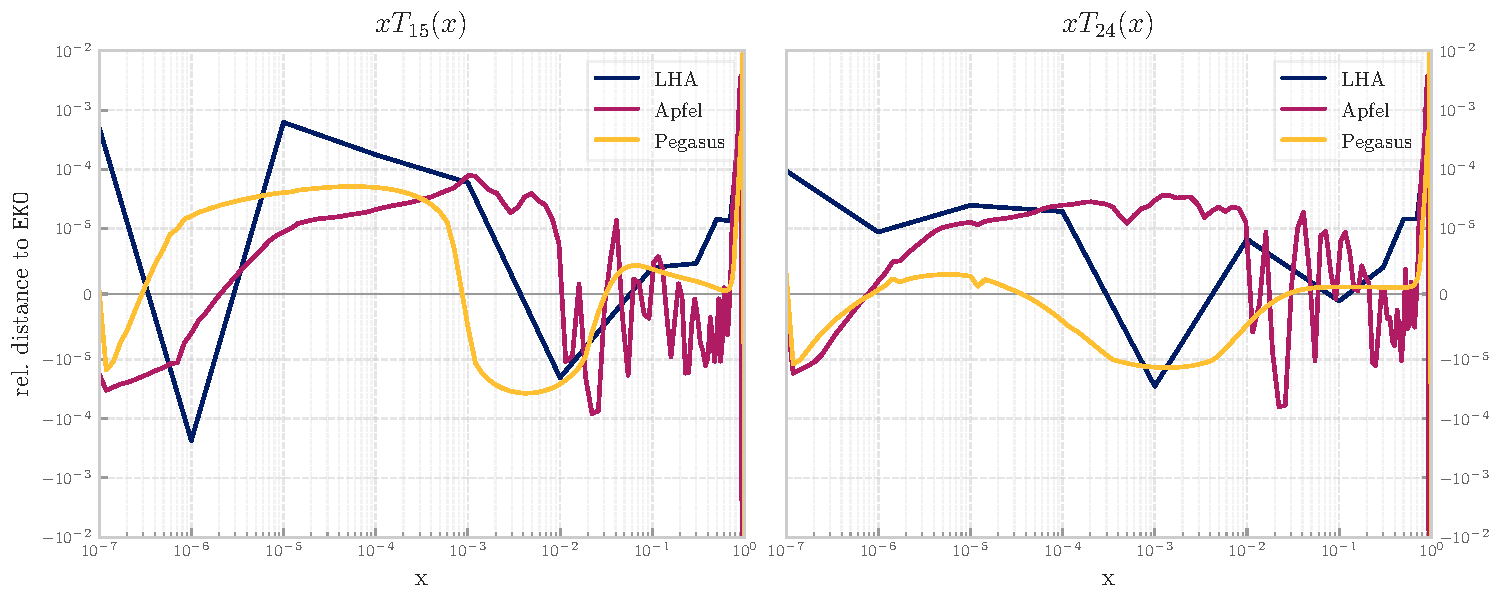
\includegraphics[width=\linewidth]{lha_bench_T15_T24.pdf}
	\end{center}
\end{frame}

\subsection{Features}
\begin{frame}{\eko{} Interpolation Error}
	\begin{center}
		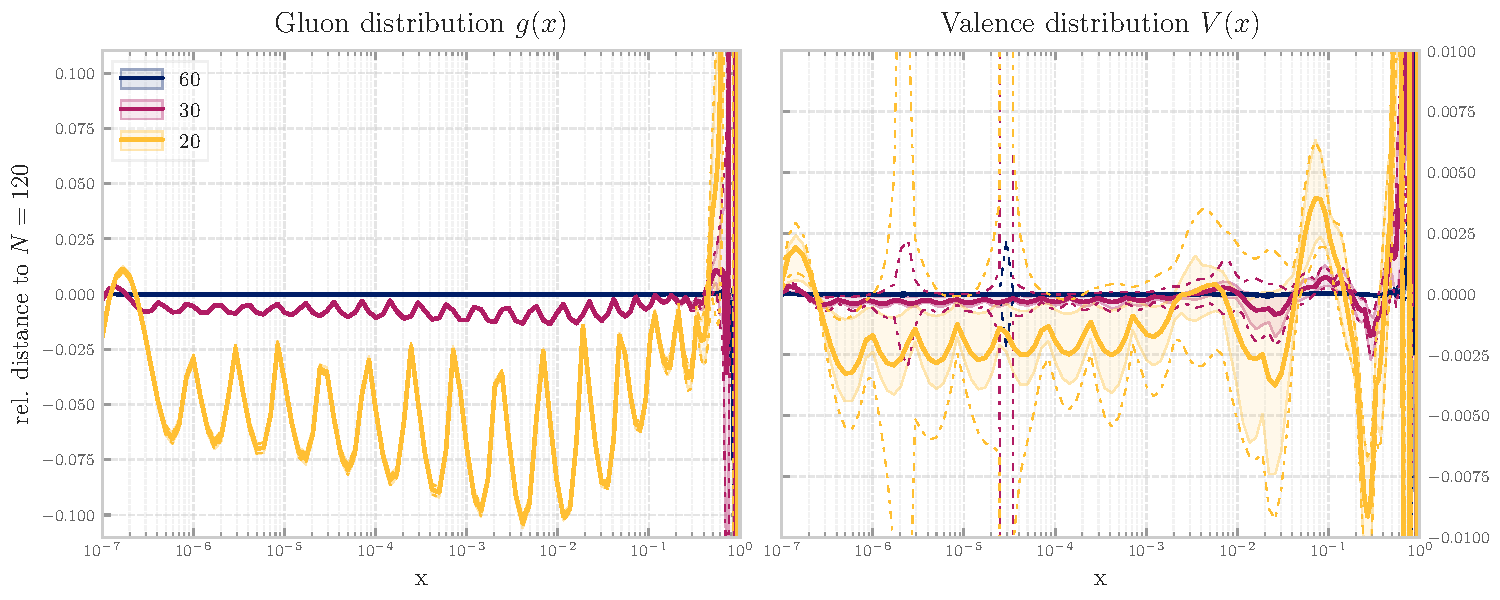
\includegraphics[width=\linewidth]{interpolation-int-ratio.pdf}
	\end{center}
\end{frame}
\begin{frame}{\eko{} Snapshot $V\leftarrow V$}
	\begin{center}
		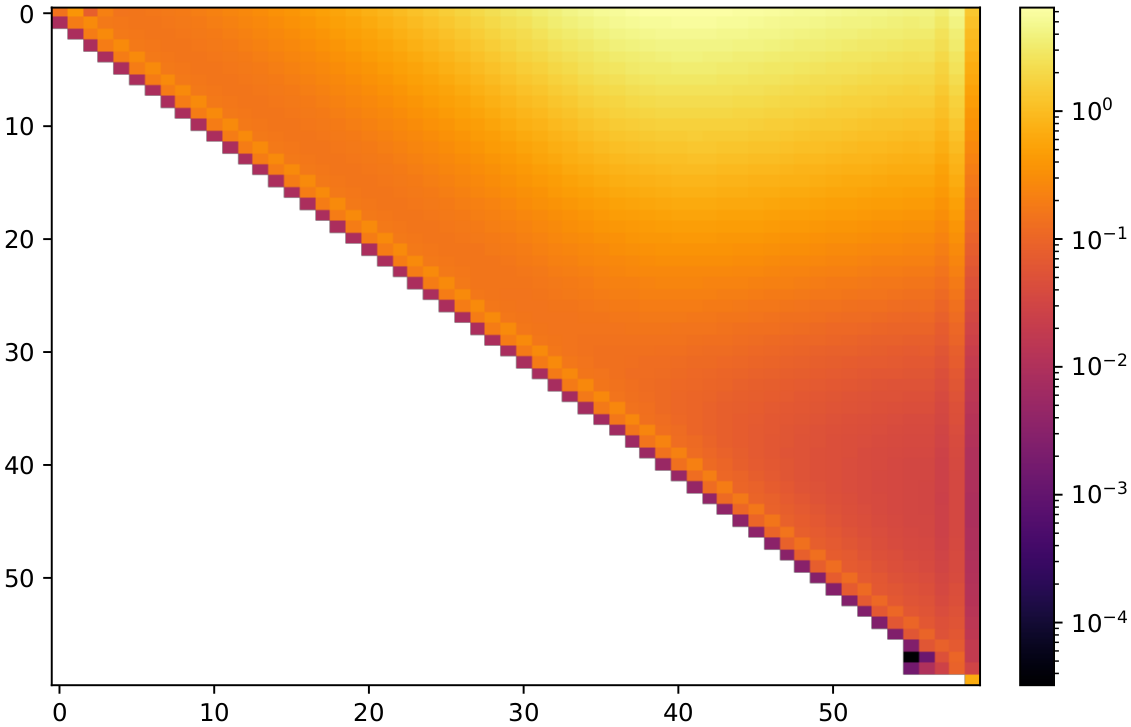
\includegraphics[width=\linewidth]{VvV.png}
	\end{center}
\end{frame}
\begin{frame}{\eko{} Backward Evolution}
	\begin{center}
		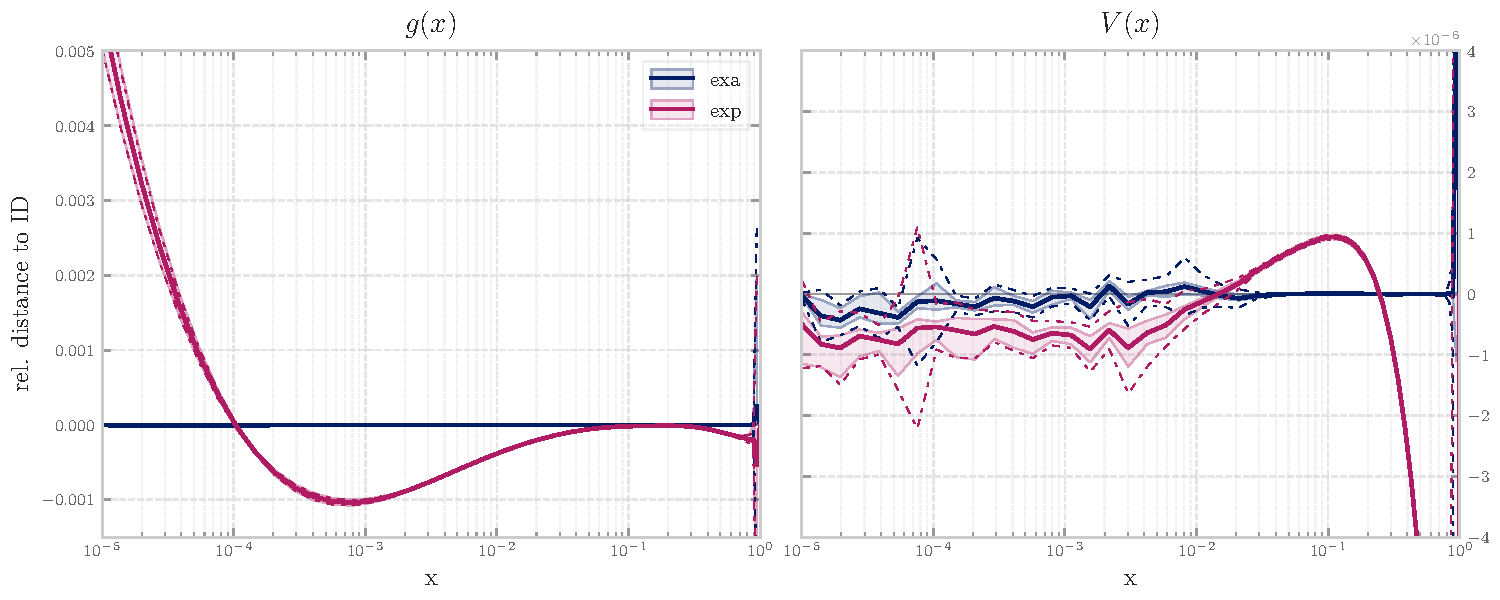
\includegraphics[width=\linewidth]{closure_test.pdf}
	\end{center}
\end{frame}

\section{Intrinsic Charm}

\begin{frame}{IC - matching perturbative order}
	\begin{center}
		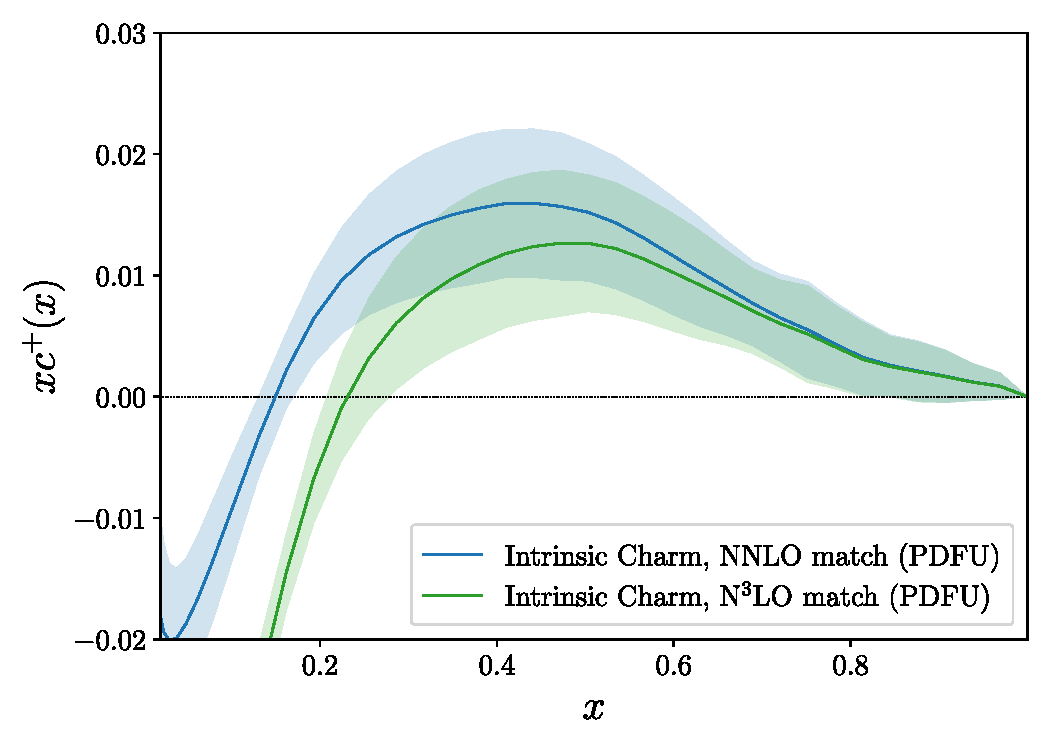
\includegraphics[width=.9\linewidth]{3fns_nnlo_n3lo}\\
                \textbf{3FNS} comparison -- \nnlo matching \textsc{vs} \nnnlo
	\end{center}
\end{frame}
\begin{frame}{IC - truncated momentum fraction}
	\begin{center}
		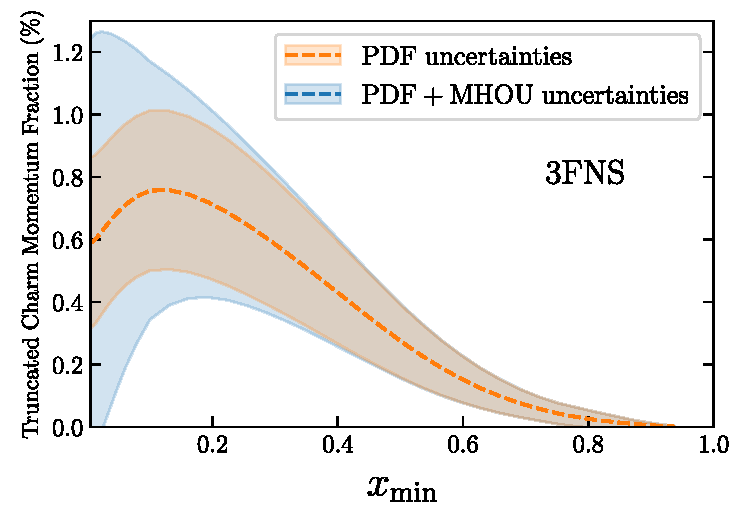
\includegraphics[width=\linewidth]{charm_momfrac_xmin_dep_3fns.pdf}
	\end{center}
\end{frame}
\begin{frame}{IC - all uncertainties combined}
	\begin{center}
		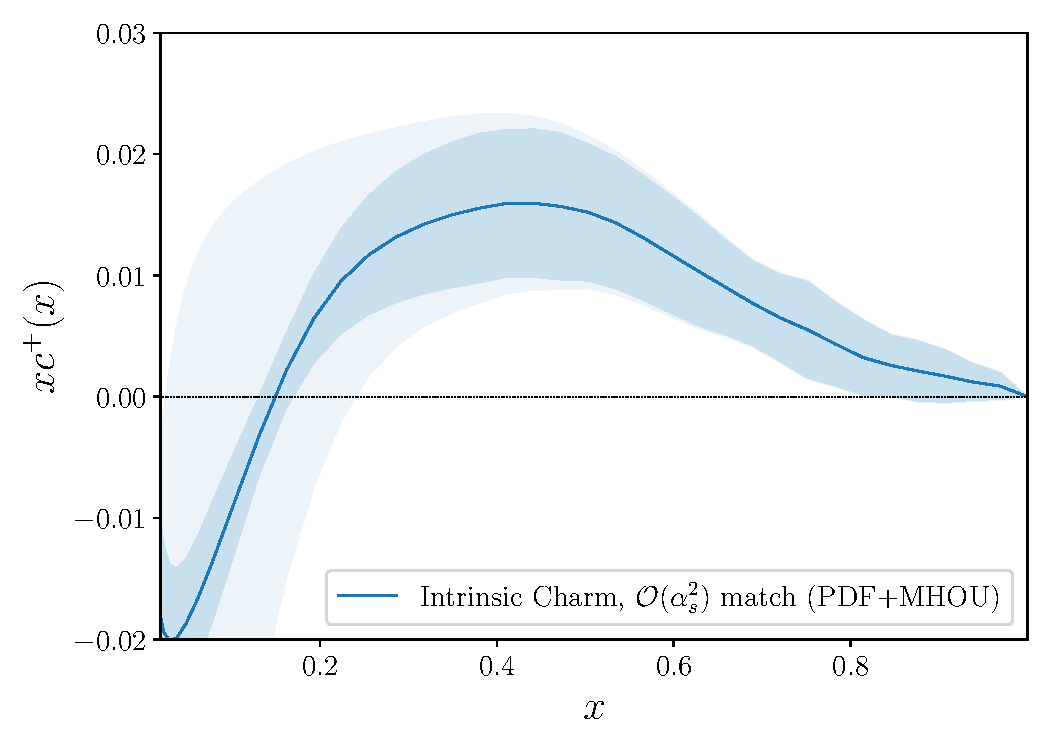
\includegraphics[width=\linewidth]{3fns_Quad_MHOU.pdf}
	\end{center}
\end{frame}
\subsection{Variations}
\begin{frame}{IC - dataset variation}
	\begin{center}
		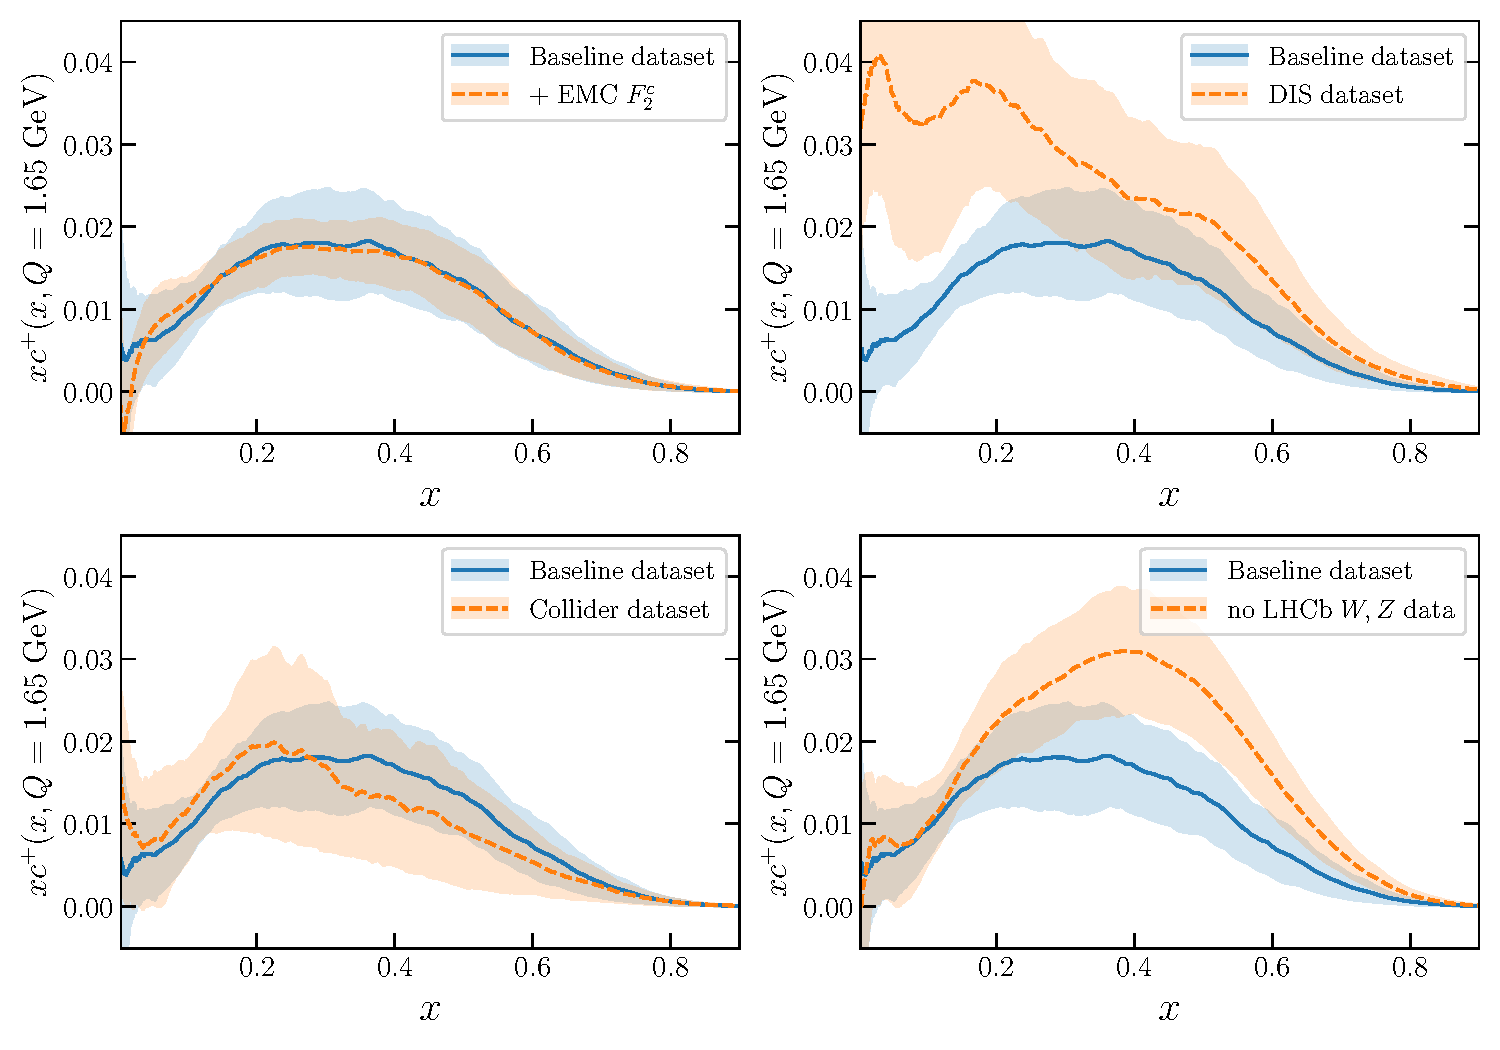
\includegraphics[width=\linewidth]{pdfplot-abscharm-dataset_dep.pdf}
	\end{center}
\end{frame}
\begin{frame}{IC - mass variation}
	\begin{center}
		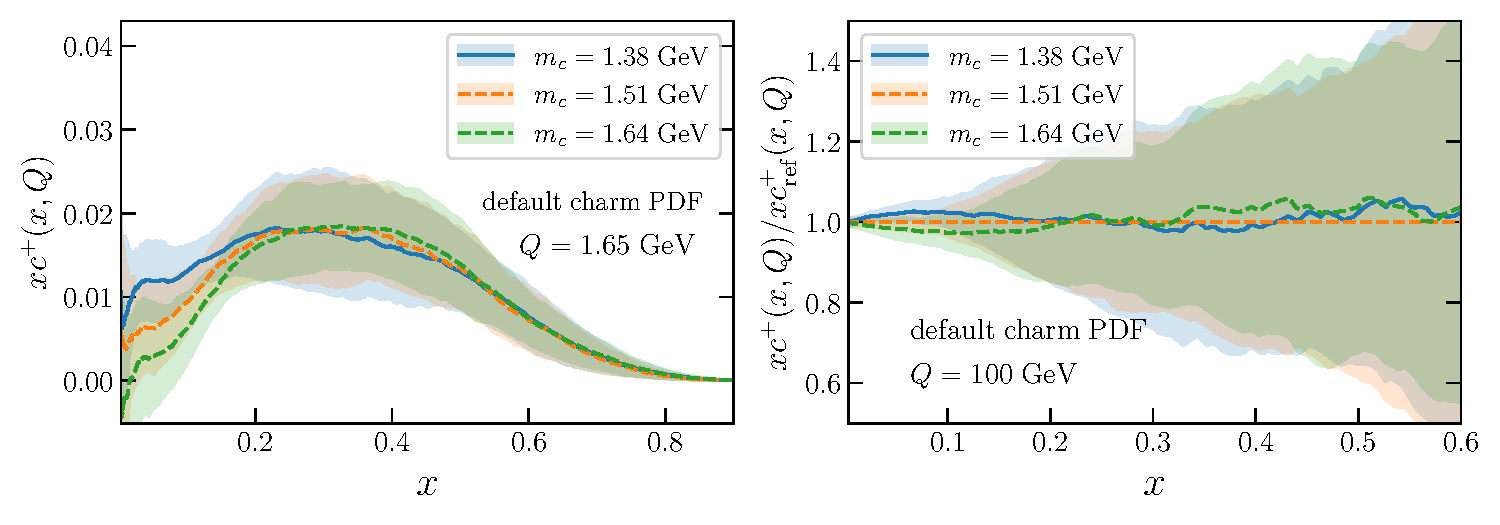
\includegraphics[width=\linewidth]{pdfplot-abscharm-mcdep.pdf}\\%
		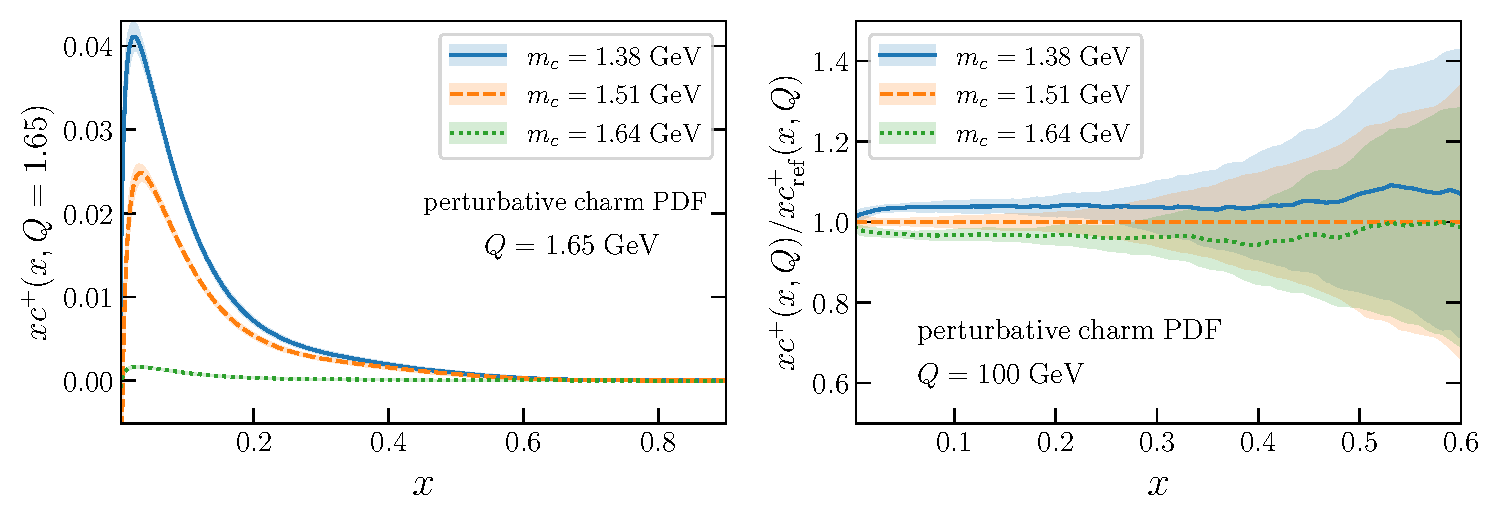
\includegraphics[width=\linewidth]{pdfplot-abscharm-mcdep-highQ.pdf}
	\end{center}
\end{frame}

\section{\yadism}
\begin{frame}{Comparison \yadism{} against \apfel{}}
	\begin{center}
		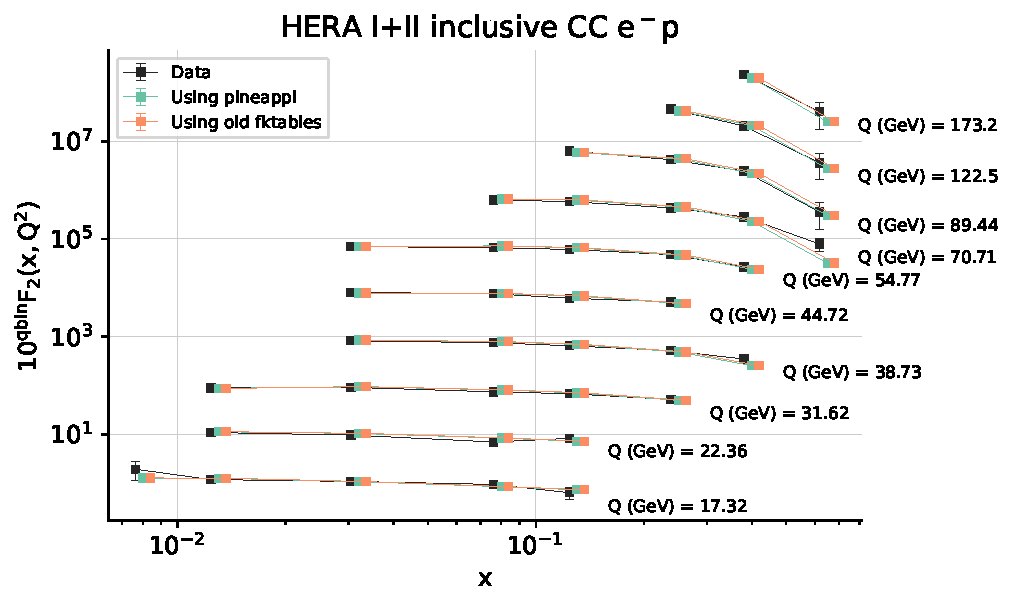
\includegraphics[width=\linewidth]{matched_datasets_from_dataspecs4_dataset_report_plot_fancy_dataspecs_0.pdf}
	\end{center}
\end{frame}
\begin{frame}{Comparison \yadism{} against \apfel{}}
	\begin{center}
		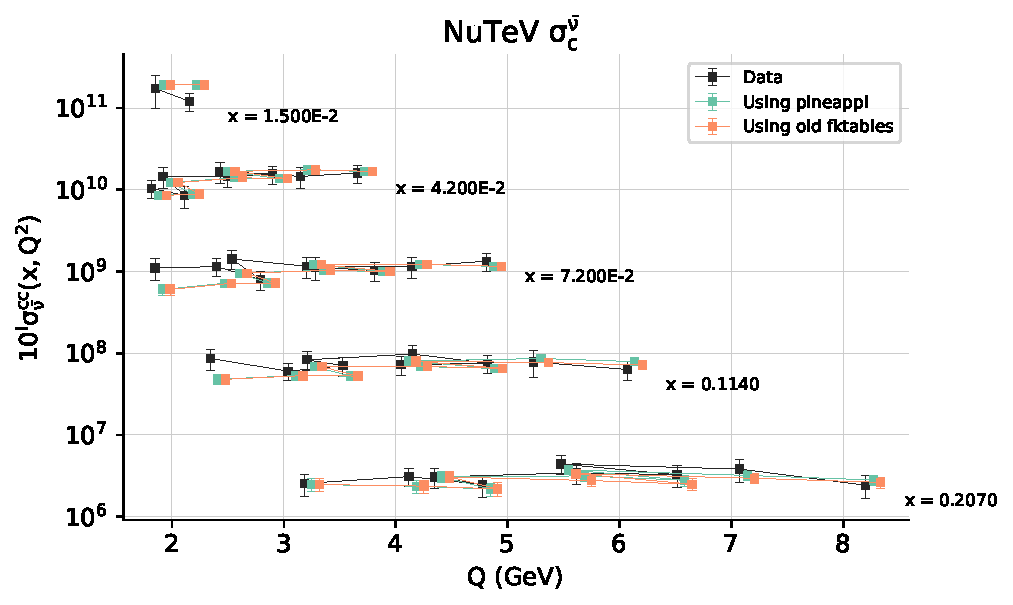
\includegraphics[width=\linewidth]{matched_datasets_from_dataspecs6_dataset_report_plot_fancy_dataspecs_0.pdf}
	\end{center}
\end{frame}

\end{document}
